\documentclass[conference]{IEEEtran}
% If IEEEtran.cls has not been installed into the LaTeX system files,
% manually specify the path to it like:
% \documentclass[conference]{../sty/IEEEtran}
\usepackage[english]{babel} 
\usepackage{longtable}
\usepackage{ifpdf}
\usepackage[table]{xcolor}

\usepackage{anysize}
\usepackage{textcomp}
\usepackage{url}
\bibliographystyle{unsrt}
\usepackage{graphics}
\usepackage{amssymb}
\usepackage{graphicx}
%\usepackage{slashbox}
\usepackage[latin1]{inputenc}
\usepackage{tikz}
\usepackage{amsmath}
\usepackage{float}
\usetikzlibrary{arrows,positioning}
% Color and strikethrough
\usepackage{color}
\usepackage{soul}

\usepackage{array}
\usepackage{makecell}

\usepackage{cite}
\usepackage{tabu}
\usepackage{caption}
\captionsetup[table]{skip=1pt}
\usepackage{paralist}
\usepackage[a4paper, total={7in, 9in}]{geometry}


%\usepackage{sectsty}
% correct bad hyphenation here
\hyphenation{op-tical net-works semi-conduc-tor}


\begin{document}
 \graphicspath{{./}{./fig/}}
%
% paper title
% Titles are generally capitalized except for words such as a, an, and, as,
% at, but, by, for, in, nor, of, on, or, the, to and up, which are usually
% not capitalized unless they are the first or last word of the title.
% Linebreaks \\ can be used within to get better formatting as desired.
% Do not put math or special symbols in the title.
\title{Design of ASIPs for Approximate Computing}


% author names and affiliations
% use a multiple column layout for up to three different
% affiliations
\author{\IEEEauthorblockN{Daniel Moya S\'anchez}
\IEEEauthorblockA{Computer Engineering Academic Area\\
Instituto Tecnol\'ogico de Costa Rica\\
Email: danielmscr1994@gmail.com}}

% make the title area
\maketitle

% As a general rule, do not put math, special symbols or citations
% in the abstract
\begin{abstract}
IT systems have been facing certain problems, among them the cost in area, power and execution time, which
restrict the performance of a chip. Application-Specific Instruction Processors (ASIPs), a solution
coming from the approximate computing area, is a design paradigm that proposes a reduction in the accuracy
or precision of the computation to obtain opportunities for improvement in terms of consumption of
area, power and execution time. This paper evaluates the design of Application-Specific Instruction Processors (ASIPs)
for error-tolerant applications in three specific applications, through the use of ASIPMeister and Dlxsim tools, which
allow the synthesis required for a processor's hardware with its Instruction Set Architecture (ISA). Reductions
in the total cycles were found for almost 10\%, 50\% and even 100\% compared to the original version, while
adding minimal area and power requirements; which prove that approximate computing and more specific ASIPs,
can bring improvements and allow the customization of hardware for special instructions. 
\end{abstract}


\IEEEpeerreviewmaketitle



\section{Introduction}

The Information Technology (IT) systems seek to give a better quality of
life to people. In this task, these systems have been facing
certain problems, among them the cost in area, power and execution time, which
restrict the performance of a chip. Ideally, an application should fit the
real needs of the user and, in general, of the area of application, so that an optimal
use of resources is achieved. Currently, processor design is not only focused on
having more performance but also having an appropriate resource management;
however, some challenges in this field are given by physical limitations,
for example:

\begin{compactitem}
 \item the electrical characteristics of the CMOS transistors, which
 restrict the emergy consumption in embedded systems and which is an issue
 that designers should consider for specific purpose
 components in processors;
 

 \item the memory wall, which corresponds to the difference between the growth
 of the processing capacity versus the speed of data gathering
 from memory;

 \item and the utilization wall, which limits the maximum use of hardware
 simultaneously due to the heat dissipation capabilities of a system.
\end{compactitem}

In order to face the problems mentioned above, an area of
current research corresponds to approximate computing, a
design paradigm that proposes a reduction in the accuracy or precision of the
computation to obtain opportunities for improvement in
area, power and execution time. To apply this paradigm, it is necessary to
identify error-tolerant applications and determine, in a specific manner,
which sections or functions within these can be replaced by
approximate versions, so that a balance can be obtained between the quality
of the output and the general consumption of resources.

This paper evaluates the design performance, in area, power and execution time, of ASIPs
for error-tolerant applications. For this purpose, three different error-tolerant applications
were evaluated and then, for each one, an special instruction, that reflects a recurrent operation 
in the original code, was implemented. Finally, the performance of each optimization
was evaluated agaisnt the original version to determine the impact of the designed ASIPs.

Since translating a whole application from the C programming language to assembly
code was too costly, only a smaller version which contains the key processing
was developed for testing purposes. 


\section{Context and background}

In the current era where sophisticated applications are widely used (e.g. GPS systems, 
speech recognition, etc.) approximate computing helps delivering acceptable
output while keeping metrics such as response time or energy efficiency at better levels. 
Approximate computing gives the freedom to tradeoff certain error level or allow quality degradation in the final output
of an application (e.g. noise in the output signal) for lower energy consumption, area or execution time, thus
giving the researcher a tool to adjust with the real and specific needs of a given application.
For a given error-tolerant system, the framework on figure \ref{fig:ap} can be applied to 
include the approximate computing paradigm \cite{xu2018approximate}.

\begin{figure}
\begin{center}
 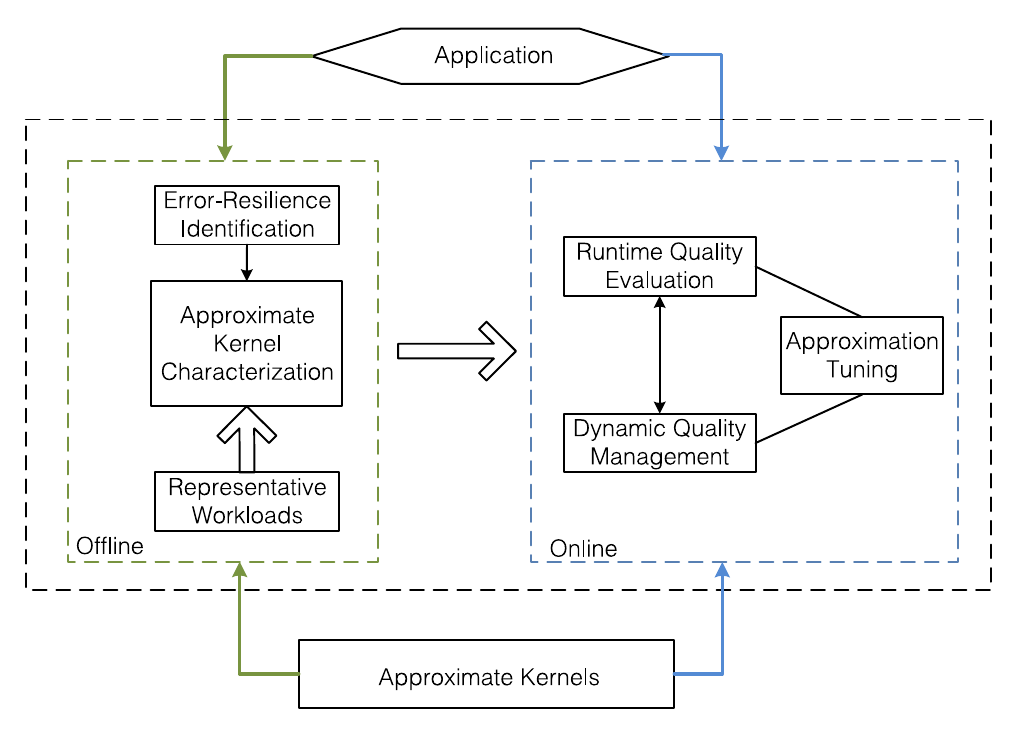
\includegraphics[width=0.5\textwidth]{APframework}
 \caption{An existing approximate computing framework \cite{xu2018approximate}} \label{fig:ap}
 \end{center}
\end{figure}

The key elements of figure \ref{fig:ap} consist of approximate kernels, which are
the implementation (techniques) of the approximate functions, these could be done at a hardware layer or at
a software layer; the identification of the error-tolerant parts
and its specific details (e.g. impact analysis); and the quality management which implies a continuos evaluation to determine
if the application meets the desired requirements \cite{xu2018approximate}.


One way to implement approximate computing is through ASIPs. An ASIP is a processor that uses an application-specific instruction set, this means 
that, although it can execute a wide range of applications, it is optimized for a 
specific one, in which the ASIP can execute with improved performance (for instance, 
energy consumption or execution time would be lower) compared to a General Purpose Proccesor (GPP).
With the use of ASIPs, instructions and even functions where there is error tolerance can be
implemented as special approximated instructions, that reduce the resource consumption 
while keeping the error from the approximation under an acceptable threshold. Although Application Specific Integrated Circuits (ASICs) show better performance 
results, ASIPs possess more flexibility. Optimizations for an ASIP can be seen in different forms, 
including \cite{henkel2003closing}:

\begin{itemize}
 \item Instruction extension: Customized instructions can be made to extend the base Instruction Set Architecture (ISA).
 
 \item Inclusion or exclusion of predefined blocks: Not only specific software can be added 
 to extend an architecture but also customized hardware in the form of specialized blocks; 
 also, regular blocks not used can be excluded.
 
 \item Parameterization: Certain variables, such as cache sizes or number of registers, can 
 be customized to adjust for a specific application.
\end{itemize}

ASICs represent a hardware solution to a problem which is very limited and have high 
costs and a high time-to-market, but achieve the greatest performance. Contrary, GPPs 
are seen as a software solution which are very flexible but they are the least efficient. ASIPs
are in the middle of these two as they balance flexibility and performance to have a 
good trade-off between those variables. 


The relationship between GPPs, ASIPs, and ASICs is shown in figure \ref{fig:gaa}.
Approximate computing can also be implemented on GPPs, due to their extremely flexible nature,
however, because they are designed for any kind of computation, it falls on the programmers, or compilers, not on specialized hardware modules,
to make the performance of software running on these systems as high as possible. On the other hand, since ASICs are a pure hardware solution,
approximate hardware modules would be difficult to manage in terms of quality evaluation,
this could cause high cost of development, since the hardware would not be programmable. ASIPs can adjust to specific requirements of
a given application (through extended instructions) so that a better balance of cost savings and 
amount of error is achieved. This project focuses on that goal; to design ASIPs for a set 
of error-tolerant applications.


\begin{figure}
\begin{center}
 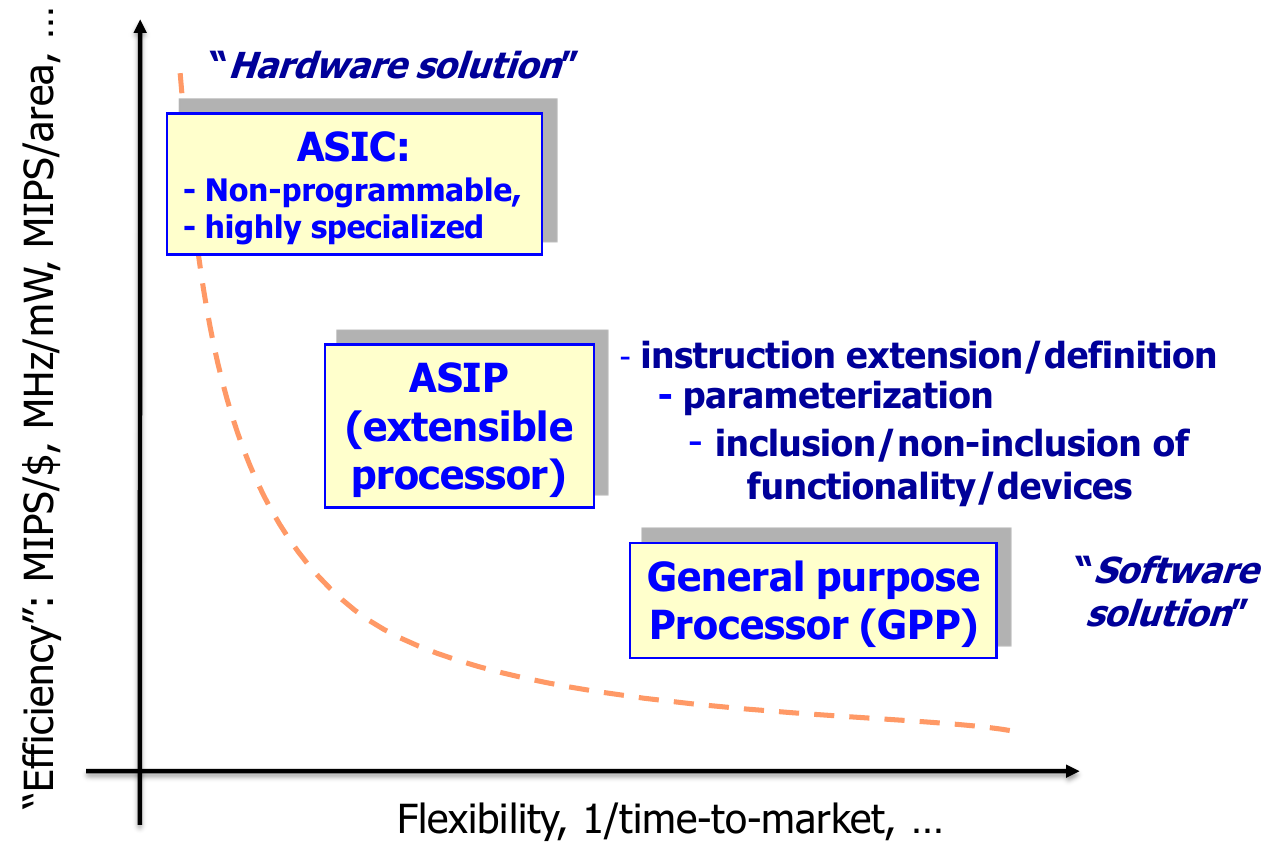
\includegraphics[width=0.5\textwidth]{GPP-ASIP-ASIC}
 \caption{Comparison between GPPs, ASIPs, and ASICs. Taken from \cite{henkel2006design}} \label{fig:gaa}
 \end{center}
\end{figure}




\section{Design of the ASIPs}


As explained before, an ASIP is able to execute a wide range of operations but also some specialized instructions
for an specific application. Following this scheme, a general processor with common instructions (for example add,
substract, shift, among others) was used, an one specific instruction was added for each different selected application.

The three aproximate applications found were K-Means, K-Nearest Neighbors (KNN) and the Sobel filter. 
All the special instructions correspond to new assembly instructions of arithmetic tpye, which modify the Instruction Set Architecture (ISA). For the K-Means
application, the special instruction \emph{eucl} was implemented, which executes part of the euclidean distance operation,
as follows (considering \emph{rd} as the destination register, \emph{rs0} and \emph{rs1} as the registers with the input values):

\begin{align}
 rd = (rs0 - rs1)^2
\end{align}

At a hardware level, this instruction uses a combinatorial block (the ALU is not used), consisting in an adder (which executes a substraction when the second input
is negated) and a multiplier.

For the KNN application, the special instruction \emph{absv} was implemented, which executes a subtract operation with an absolute result, 
which is used frequently in the KNN algorithm (the euclidean distance remains the main operation in this algorithm too). At at high abstraction level,
this operation executes:

\begin{align}
 rd = rs0 > rs1 ? rs0-rs1 : rs0-rs1
\end{align}
At a hardware level, a simple adder (which executes a substraction) and a mux are used, in an additional combinatorial block.

For the last application, the Sobel filter, the special instruction \emph{sob} was developed, which allows computing the following operation in a single cycle:

 \begin{align}
  rd = rs0^2 + rs1^2
 \end{align}

The operation described in (3) allows the execution of two multiplications and an addition operation, which is used frequently in the Sobel algorithm. Other operations 
in this algorithm could not be turned into special instructions (for example, a matrix multiplication) because they require more than two paremeters. 
At a hardware level, this instructions requires two multipliers and one adder (the ALU is not used).

To test these special instructions, small assembly codes were developed which consist in the execution of the selected operation through an array of 100 elements. For the three
approximate applications found, two assembly codes were developed, one with where the special instruction is used and another equivalent with common assembly instruction to 
execute the same as the special instruction.

\section{Analysis of Results}

Each assembly code for the approximate applications (both the version using the special instruction and the version without it) were simulated in order to obtain the total number of cycles
and integer operations (for example, multiplications, additions, etc.) for comparison. At a hardware level, the architecture with the additional specialized hardware was simulated in order
to obtain data to compare between the optimized version and the original processor, in terms of area (slices and LUTs) and power. 


For the \emph{eucl} instruction, an 8\% lower total number of cycles was achieved with the optimized version.

\begin{table}[h!]
\begin{center}
\caption{Cycles comparison for the \emph{eucl} instruction}
\resizebox{0.5\textwidth}{!}{\begin{tabular}{|c|c|c|c|} 
 \hline
\multicolumn{2}{|c|}{With the \emph{eucl} instruction} &\multicolumn{2}{|c|}{Without the \emph{eucl} instruction}\\ \hline
Total Cycles	&\# Integer Operations	&Total Cycles	&\# Integer Operations	 \\ \hline
4730	&1128	&5130	&1528 \\ \hline
 \end{tabular}}
\label{tab:schd}
\end{center}
\end{table}

\begin{table}[h!]
\begin{center}
\caption{Area comparison for the \emph{eucl} instruction}
\resizebox{0.5\textwidth}{!}{\begin{tabular}{|c|c|c|c|c|c|c|c|} 
 \hline
\multicolumn{4}{|c|}{With the \emph{eucl} instruction} &\multicolumn{4}{|c|}{Without the \emph{eucl} instruction}\\ \hline
\# Slices	&\% Slices	&\# LUTs	&\% LUTs	&\# Slices	&\% Slices	&\# LUTs	&\% LUTs \\ \hline
3998	&5\%	&6384	&9\%	&3990	&5\%	&6199	&8\% \\ \hline
 \end{tabular}}
\label{tab:schd}
\end{center}
\end{table}

\begin{table}[h!]
\begin{center}
\caption{Power comparison for the \emph{eucl} instruction}
\resizebox{0.5\textwidth}{!}{\begin{tabular}{|c|c|c|c|c|c|} 
 \hline
\multicolumn{3}{|c|}{With the \emph{eucl} instruction} &\multicolumn{3}{|c|}{Without the \emph{eucl} instruction}\\ \hline
Total Power 	&Dynamic Power 	&Quiescent Power 	&Total Power 	&Dynamic Power 	&Quiescent Power  \\ \hline
1497 mW	&335 mW	&1163 mW	&1492 mW	&330 mW	&1163 mW \\ \hline
\end{tabular}}
\label{tab:schd}
\end{center}
\end{table}


\begin{table}[h!]
\begin{center}
\caption{Cycles comparison for the \emph{absv} instruction}
\resizebox{0.5\textwidth}{!}{\begin{tabular}{|c|c|c|c|} 
 \hline
\multicolumn{2}{|c|}{With the \emph{absv} instruction} &\multicolumn{2}{|c|}{Without the \emph{absv} instruction}\\ \hline
Total Cycles	&\# Integer Operations	&Total Cycles	&\# Integer Operations	 \\ \hline
1330	&1128	&2534	&2133 \\ \hline
 \end{tabular}}
\label{tab:schd}
\end{center}
\end{table}

\begin{table}[h!]
\begin{center}
\caption{Area comparison for the \emph{absv} instruction}
\resizebox{0.5\textwidth}{!}{\begin{tabular}{|c|c|c|c|c|c|c|c|} 
 \hline
\multicolumn{4}{|c|}{With the \emph{absv} instruction} &\multicolumn{4}{|c|}{Without the \emph{absv} instruction}\\ \hline
\# Slices	&\% Slices	&\# LUTs	&\% LUTs	&\# Slices	&\% Slices	&\# LUTs	&\% LUTs \\ \hline
4058	&5\%	&6465	&9\%	&3990	&5\%	&6199	&8\% \\ \hline
 \end{tabular}}
\label{tab:schd}
\end{center}
\end{table}

\begin{table}[h!]
\begin{center}
\caption{Power comparison for the \emph{absv} instruction}
\resizebox{0.5\textwidth}{!}{\begin{tabular}{|c|c|c|c|c|c|} 
 \hline
\multicolumn{3}{|c|}{With the \emph{absv} instruction} &\multicolumn{3}{|c|}{Without the \emph{absv} instruction}\\ \hline
Total Power 	&Dynamic Power 	&Quiescent Power 	&Total Power 	&Dynamic Power 	&Quiescent Power  \\ \hline
1495 mW	&333 mW	&1163 mW	&1492 mW	&330 mW	&1163 mW \\ \hline
\end{tabular}}
\label{tab:schd}
\end{center}
\end{table}

\begin{table}[h!]
\begin{center}
\caption{Cycles comparison for the \emph{sob} instruction}
\resizebox{0.5\textwidth}{!}{\begin{tabular}{|c|c|c|c|} 
 \hline
\multicolumn{2}{|c|}{With the \emph{sob} instruction} &\multicolumn{2}{|c|}{Without the \emph{sob} instruction}\\ \hline
Total Cycles	&\# Integer Operations	&Total Cycles	&\# Integer Operations	 \\ \hline
4730	&1128	&8930	&1928 \\ \hline
 \end{tabular}}
\label{tab:schd}
\end{center}
\end{table}


\begin{table}[h!]
\begin{center}
\caption{Area comparison for the \emph{sob} instruction}
\resizebox{0.5\textwidth}{!}{\begin{tabular}{|c|c|c|c|c|c|c|c|} 
 \hline
\multicolumn{4}{|c|}{With the \emph{sob} instruction} &\multicolumn{4}{|c|}{Without the \emph{sob} instruction}\\ \hline
\# Slices	&\% Slices	&\# LUTs	&\% LUTs	&\# Slices	&\% Slices	&\# LUTs	&\% LUTs \\ \hline
4223	&6\%	&6079	&8\%	&3990	&5\%	&6199	&8\% \\ \hline
 \end{tabular}}
\label{tab:schd}
\end{center}
\end{table}

\begin{table}[h!]
\begin{center}
\caption{Power comparison for the \emph{sob} instruction}
\resizebox{0.5\textwidth}{!}{\begin{tabular}{|c|c|c|c|c|c|} 
 \hline
\multicolumn{3}{|c|}{With the \emph{sob} instruction} &\multicolumn{3}{|c|}{Without the \emph{sob} instruction}\\ \hline
Total Power 	&Dynamic Power 	&Quiescent Power 	&Total Power 	&Dynamic Power 	&Quiescent Power  \\ \hline
1495 mW	&333 mW	&1163 mW	&1492 mW	&330 mW	&1163 mW \\ \hline
\end{tabular}}
\label{tab:schd}
\end{center}
\end{table}


\section{Conclusion}


ASIP showed lower execution times while increasing the overall hardware and power at roughly 1\% compared to the original version.



\bibliographystyle{sty/plainurl}
\bibliography{references}




% that's all folks
\end{document}


